\documentclass{beamer}

\mode<presentation>{}

\usepackage[english]{babel}
\usepackage[latin1]{inputenc}
\usepackage{times}
\usepackage[T1]{fontenc}

\title[``Statistical'' Computing]
{Putting Statistics back into Statistical Computing}

\subtitle{Moving from Data Science back to Statistics}

\author[] 
{A.J.~(Tony)~Rossini}

\institute[Novartis Pharma AG and University of Washington]
{
  Quantitative Safety and Epidemiology\\
  Novartis Pharma AG \\
  Basel
  \and
  Department of Biomedical and Health Informatics\\
  University of Washington}

\date[StatComp 2014] % (optional, should be abbreviation of conference name)
{Reisensburg, 2014}

\subject{Theoretical Statistical Computing}

\begin{document}

\begin{frame}
  \titlepage
\end{frame}

\begin{frame}{Outline}
  \tableofcontents
\end{frame}


\section{Background}

\begin{frame}{Motivation}
  Languages help shape the way we think about our activities and
  actions.

  \vspace*{1cm}

  \textbf{Computer languages, doubly so.}  
  
  \vspace*{1cm}

  \textit{(by what is easy or hard to express)}

  \vspace*{1cm}

  Caveat: \textit{EVERYTHING can be written in assembly language.}
\end{frame}

\begin{frame}{Quick Rehash of Grad School}
  \begin{itemize}
  \item Probabilities: distributions, functionals on distributional
    quantities, higher order interactions, (Conditional)
    Independence/Expectation
  \item Data: Distributional, sampling, exo-/endogenous assumptions and
    selecting the best statistical procedure(s)
  \item Decision making support: models (explicit/algorithmic),
    estimation algorithms, computed results and uncertainty.
  \end{itemize}
\end{frame}

\begin{frame}{Topics relevant to this talk}{in and out of scope}


  \begin{itemize}
  \item \textbf{Out of scope:} High performance statistical computing,
    visualization, ``making the applied work faster through faster
    computation''.
  \item \textbf{In scope:} reproducibility, transparence, assessment
    of statistical procedure applicability, communication of the
    quality of the implemented data analysis (through code review).
  \end{itemize}

  Goal: make the time spent by a human of higher value and quality
\end{frame}

\section{Statistical Computing or Data Analysis Computing?}

\begin{frame}{The Missing Link}{what is not missing}
  Much work on computing systems tries to put or map the domain
  concepts/information into the system (bioinformatics, travel, social
  relationships).  

  In evaluating \textbf{data analysis} computing systems, what of
  statistics can be found?
  \begin{itemize}
  \item algorithms
  \item probability
  \item modeling tools
  \end{itemize}
  what domain support is missing?
\end{frame}

\begin{frame}{The Missing Link}{It is difficult to find}
  Starting a research view of statistics, where are
  \begin{itemize}
  \item assumptions for:
    \begin{itemize}
    \item  data (partially),
    \item  models (often),
    \item  procedures (almost always)
    \end{itemize}
  \item Separation of data, model, and inferential
    (estimation,test,algorithm) routines.

    (R: partial data separation, but models often explicitly linked to
    data, not quite but almost first-class objects)
  \item Specification and persistence of concepts across sessions.
  \end{itemize}
\end{frame}

\begin{frame}{Data Analysis vs. Statistics}

  \begin{itemize}
  \item Computations for data analysis, supported using statistics
    (Current State)
  \item How can one have statistical ``research'' supported through
    computation?
  \item How can statistical research and knowledge be better
    incorporated into the computation?
  \end{itemize}
\end{frame}


\begin{frame}{Data Analysis vs. Statistics}{Examples}
  \begin{itemize}
  \item Making Data frames statistical objects
  \item Ontologies for statistical analysis specification
  \item Computable Calculus for probability
  \item Specification of analysis strategies: \textit{Extreme Statistical Programming}
  \item Grammar of Graphics (2d, 3d, dynamic, interactive)
  \item Characteristisation of procedures (what breaks, what works,
    direct access to examples)
  \item ...
  \end{itemize}
  (not all by me, not all discussed here)
\end{frame}

\section{Putting Statistical Concepts back}

\subsection{Data Frames}

\begin{frame}{Data Frames}{(conditional) Independence}

  \begin{itemize}
  \item Should one need to go between long and wide formats?
  \item Is long/wide just a computational convenience, or is it a
    statistical issue (conditional independence)
  \end{itemize}
  \begin{table}
    \centering
    \begin{tabular}{c|c|c|c|c}
      \hline
      ID & Gender & Network     &  kinetics & treatment \\ 
      &        & (node,edge) & (measures,times) & treatment \\ 
      \hline
      US2349 & Male & (4, 5) & (3,4) & TXT1 \\
      \hline
      IN549  & Male & (2, 1) & (2,8) & TXT2 \\
      \hline
      
    \end{tabular}
  \end{table}

\end{frame}

\subsection{Ontologies}

\begin{frame}{Expressing Concepts}{so we can compute with them}
  Ontologies (restricted vocabularies) allow for knowledge representation
  \begin{itemize}
  \item Example:  If label \textbf{INFPROC32}, then it must be a
    t-test (but which? might need a term for the variance computation)
  \item Procedures:
    \begin{itemize}
    \item appropriateness (how well does the scientific question and data match
      the proposed procedure)
    \item discovery (are there any other procedures to consider?
    \item confirmation, appropriateness (matching up performance characteristics)
    \end{itemize}
  \item Assumptions: managing \textit{appropriateness}
  \end{itemize}
\end{frame}

\begin{frame}{Example Ont}
  \begin{figure}
    \centering
    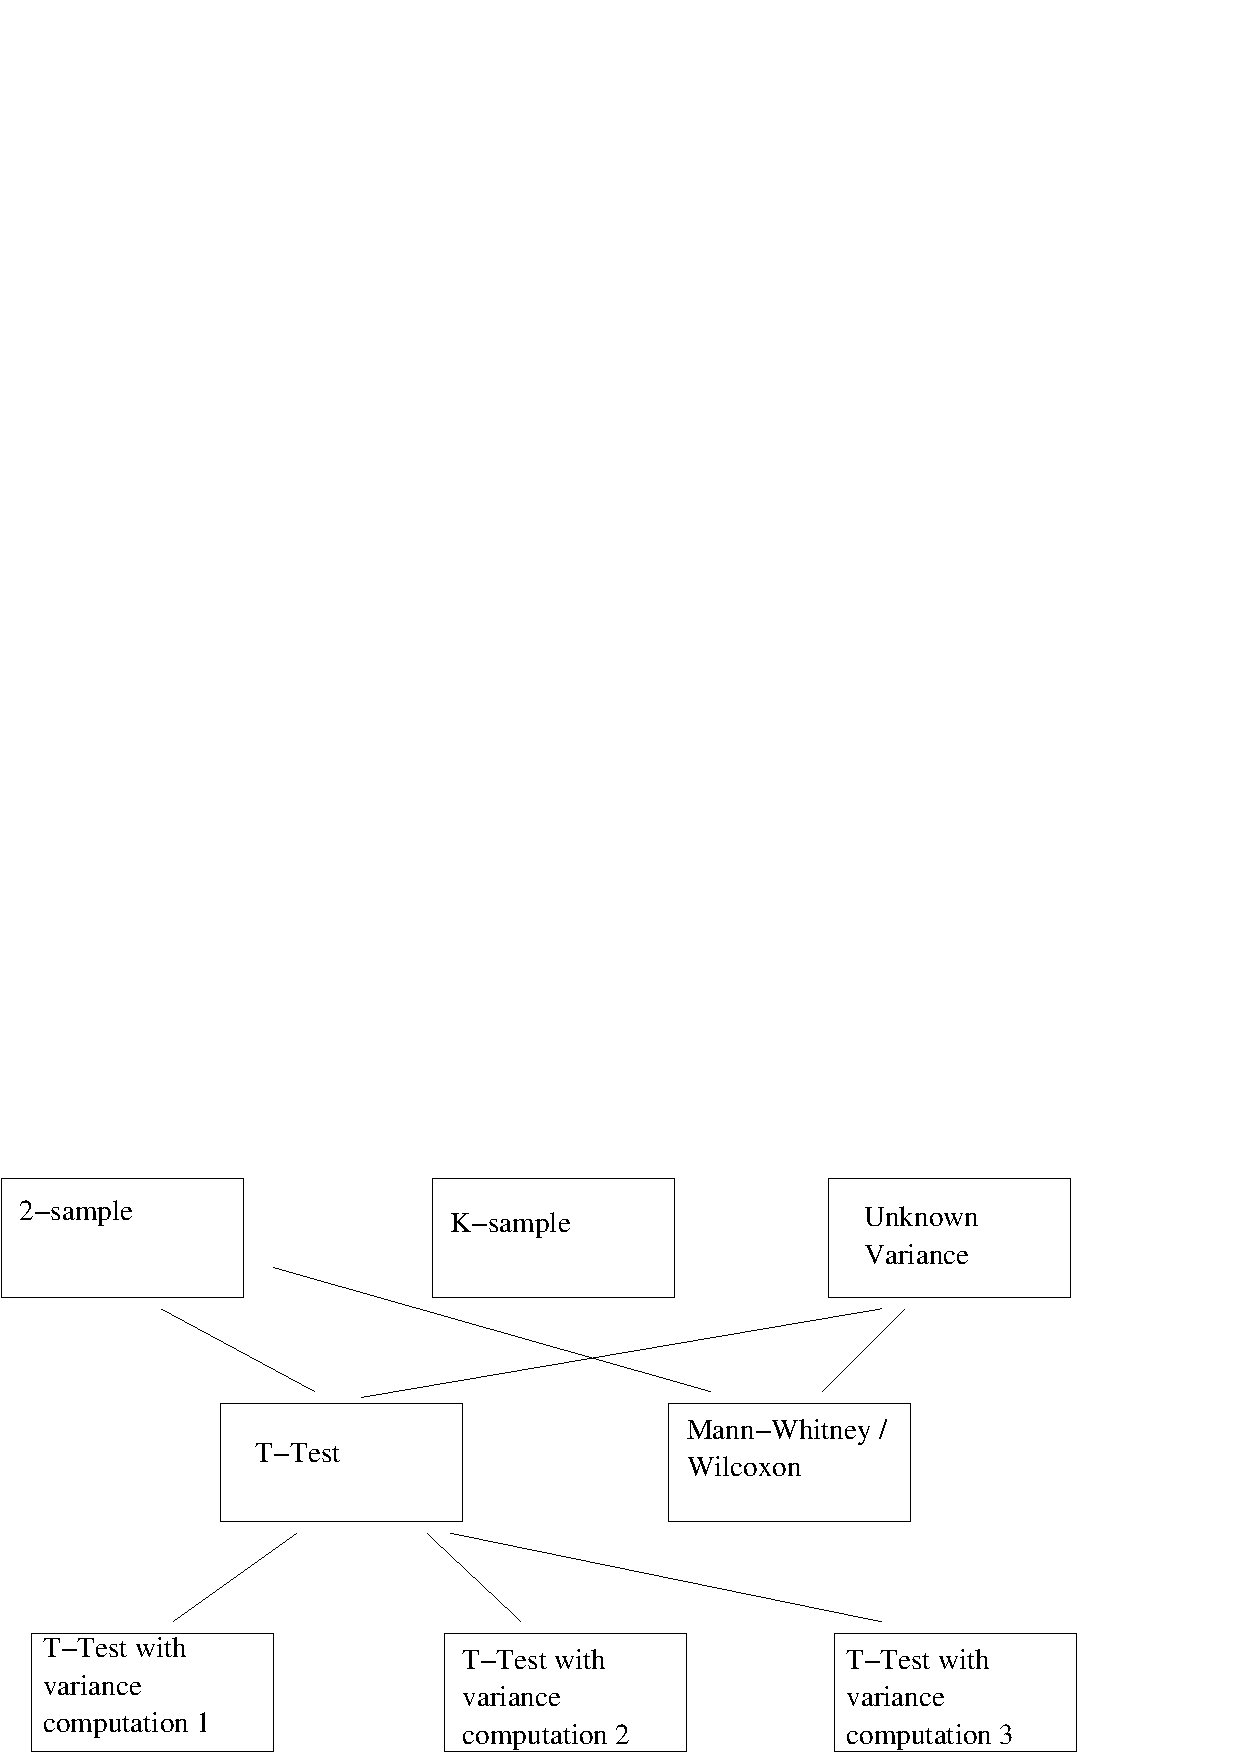
\includegraphics[width=3in,height=3in]{./ont.pdf}
  \end{figure}
\end{frame}

\begin{frame}[fragile]{The blind men and the Elephant}
\begin{verbatim}
;; -> list of results from proc
(fnmap #'stat-procedure1
       '(:data dataset
         :extra-assumptions (list of assumptions)))

;; -> list of list of...
(fnmap (list #'stat-procedure1 #'stat-procedure2)
       '(:data dataset
        :extra-assumptions (list of assumptions)))
\end{verbatim}
ex: t-test, wilcoxon, z-test

assumptions are from the ontology terms.
\end{frame}

\begin{frame}{Putting Pieces Together}{(some of them)}
\end{frame}

\begin{frame}{Extreme Statistical Programming}
  Extreme or Agile programming
  \begin{itemize}
  \item Working in pairs
  \item Solving small pieces of the puzzle
  \item Flexible (changing) and computable  specification (ontologies)
  \end{itemize}
  Perhaps only a small component is flexible.
  \vspace*{1cm}
  (business case; corporate statistical results)
\end{frame}

\begin{frame}{Business Case}{Global Analysis}
  \begin{enumerate}
  \item Scope the problem in Basel
  \item Start the analysis in the USA
  \item Continue the analysis in China/India
  \item Finish up the results in Turkey
  \item Present Results in Basel
  \end{enumerate}
\end{frame}


\begin{frame}{A Data Analysis ``Assembly line''}
  As seen by business case example, one could consider:
  \begin{enumerate}
  \item Scope the problem with the subject investigator
  \item Design the approach (maybe a study, but at least the approach)
  \item Implement the design
  \item Operate study (with or without intervention or adaptation)
  \item Analysis of results
  \item Generation of artifacts
  \end{enumerate}
  Extreme approach could be applied to 1,2,4,5.

  Ontologies would be required to support communication between data
  analysts
\end{frame}


\section*{Summary}

\begin{frame}{Summary}

  Goal: to find and implement concepts which improve the production of
  statistically oriented results to drive better quality decision
  making. 

  Goal: to support the awareness of the discipline as an essential
  component of quantitative knowledge generation. 

  Another goal is to increase the quality of such work.
  \begin{itemize}
  \item Doing statistical analyses is well supported by current
    computing systems.  Doing statistics (research, R\&D) is not.
    Translating research into practice is a manual, one-off process.
  \item Good theory is required for good practice.  Good practice
    drives better theory.
  \item Who cares about big data?  There are still many open (but very
    challenging) problems in \textbf{small data / big decision}
  \end{itemize}
\end{frame}

\begin{frame}{Outlook}
  
  \begin{itemize}
  \item Ideas are currently being implemented in Common Lisp
    Statistics (perhaps next year's talk) 
  \item They can be implemented in R, and in Standard Operating
    Procedures, and in .... (but that is for someone else).
  \item They might be useful.
  \end{itemize}
  Or not.  
\end{frame}

% \begin{frame}{New motivation}{What is is the difference between a...}
%   % - A title should summarize the slide in an understandable fashion
%   %   for anyone how does not follow everything on the slide itself.

%   \begin{itemize}
%   \item a statistician who fits a logistic regression model to
%     categorical covariates
%   \item a computer scientist who fits a neural network
%   \item a data scientist predicting binary responses
%   \end{itemize}
%   ?? Not much.

%   \texttt{Let's not argue on small matters: Many people take data,
%     generate information, and try to communicate knowledge.}
% \end{frame}

\end{document}


